\documentclass[master.tex]{subfiles}
 
\begin{document}



To treat the domain boundaries ghost cells are implemented. Currently the simulation needs two ghost cells into every direction. The memory and performance impact is discussed in the \textit{Computer Science} section.
\subsection{X-Direction}
In X-Direction (i. e. polodial distance) Dirichlet boundaries are implemented. This is achieved using the ghost cells and simply setting them once. To reduce gradients at the boundaries further actions have to be taken at the x boundaries (\autoref{sec:components-external}).
\subsection{Y-Direction}
In Y-Direction (which is perpendicular to X but not in torodial direction) closed boundary conditions are implemented. One of the consequences is that there is an \textit{in and out flow} of vorticies simulating turbulence incoming from the not simulated area of the polodial slice. \todo{find reference for that}The resolution in Y-Direction needs to be choosen carefully such that vorticies that are mirrored to the opposite do not interfere with themselfes. 
\subsection{Z-Direction}
In Z-Direction there is a differentiation whether the X-coordinate lies in/on or outside the separatrix.
\paragraph{In/On Separatrix}
Here we assume closed field lines and thus employ closed boundary conditions.
\paragraph{Outside of Separatrix}
To simulate \todo{Ref-Ribero-Scott} divertors outside the separatrix so called \textit{limiters} are simulated by not connecting the $z=0 \And z=n_z$ planes but rather using open boundary conditions for the densities and potential, and Dirichlet boundary conditions for the velocities. The situation is illustrated in \autoref{fig:boundary_conditions_z}
\begin{figure}[ht]
    \centering
    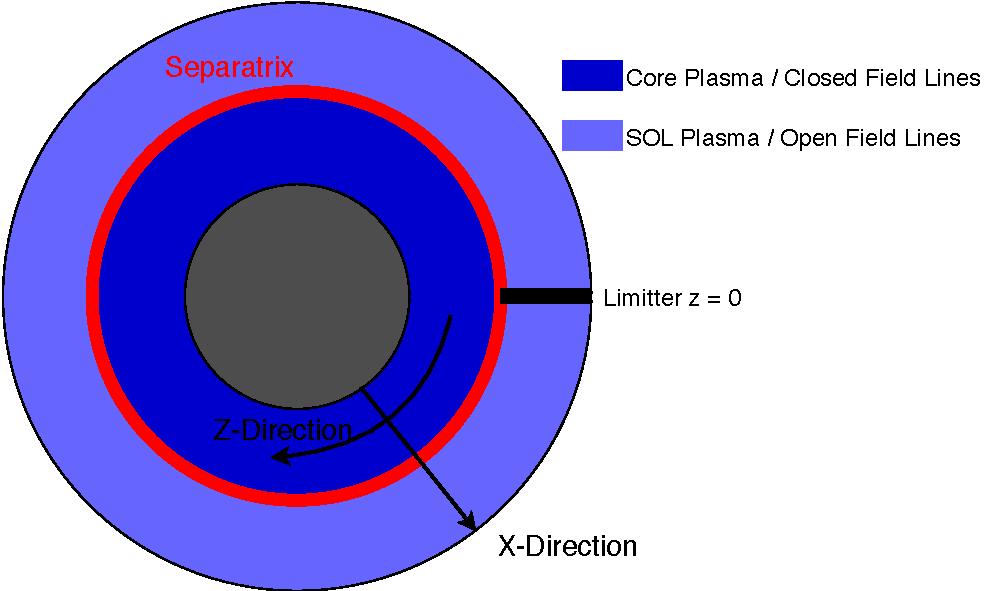
\includegraphics[width=\linewidth]{pdfs/boundary_conditions_z.pdf}
    \caption{Visualization of tokamak with separatrix and limiter}
    \label{fig:boundary_conditions_z}
\end{figure}

\end{document}